\definecolor{BPBlue}{HTML}{356F9F}
\definecolor{BPOrange}{HTML}{B66718}

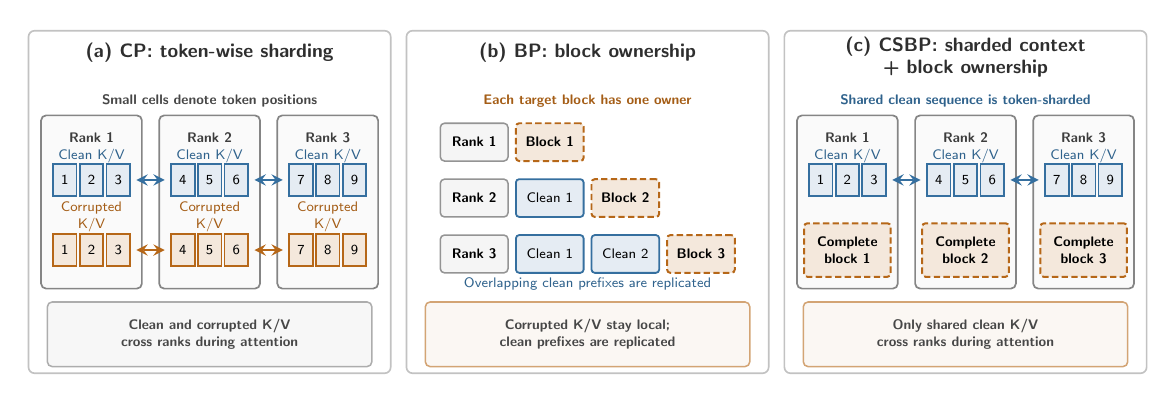
\begin{tikzpicture}[
    x=1cm,
    y=1cm,
    font=\sffamily\tiny,
    panel/.style={draw=black!24, rounded corners=2.2pt, line width=0.6pt,
                  minimum width=4.60cm, minimum height=4.35cm},
    clean/.style={draw=BPBlue, fill=BPBlue!13, rounded corners=1.2pt,
                  line width=0.65pt, minimum height=0.48cm,
                  inner xsep=0.05cm, inner ysep=0.03cm, align=center},
    corrupt/.style={draw=BPOrange, fill=BPOrange!15, rounded corners=1.2pt,
                    dash pattern=on 2.3pt off 1.2pt, line width=0.72pt,
                    minimum height=0.48cm, inner xsep=0.05cm,
                    inner ysep=0.03cm, align=center},
    ranklabel/.style={draw=black!42, fill=black!4, rounded corners=1.5pt,
                     line width=0.55pt, minimum width=0.86cm,
                     minimum height=0.48cm, inner xsep=0.05cm,
                     inner ysep=0.03cm, align=center,
                     font=\sffamily\tiny\bfseries},
    rankframe/.style={draw=black!48, fill=black!2, rounded corners=1.8pt,
                     line width=0.62pt, minimum width=1.28cm,
                     minimum height=2.20cm},
    summary/.style={draw=black!32, fill=black!3, rounded corners=1.7pt,
                    line width=0.55pt, minimum width=4.12cm,
                    minimum height=0.82cm, text width=3.88cm,
                    inner xsep=0.08cm, inner ysep=0.04cm, align=center}
]

% Equal panel frames keep the ownership progression visually comparable.
\node[panel] at (2.40,2.18) {};
\node[panel] at (7.20,2.18) {};
\node[panel] at (12.00,2.18) {};

\node[font=\sffamily\scriptsize\bfseries, text=black!82]
      at (2.40,4.08) {(a) CP: token-wise sharding};
\node[font=\sffamily\scriptsize\bfseries, text=black!82]
      at (7.20,4.08) {(b) BP: block ownership};
\node[font=\sffamily\scriptsize\bfseries, text=black!82, align=center]
      at (12.00,4.02) {(c) CSBP: sharded context\\+ block ownership};

% (a) Conventional CP transports both streams, regardless of cross-block reuse.
\foreach \x/\r in {0.90/1,2.40/2,3.90/3} {
    \node[rankframe] at (\x,2.18) {};
    \node[font=\sffamily\tiny\bfseries, text=black!76]
          at (\x,3.00) {Rank \r};
    \node[text=BPBlue!88!black] at (\x,2.76) {Clean K/V};
    \node[text=BPOrange!90!black, align=center]
          at (\x,1.99) {Corrupted\\K/V};
    % Individual cells denote token positions, not denoising blocks.
    \foreach \i in {1,2,3} {
        \pgfmathtruncatemacro{\tokenpos}{3*(\r-1)+\i}
        \node[draw=BPBlue, fill=BPBlue!13, line width=0.65pt,
              minimum width=0.30cm, minimum height=0.40cm, inner sep=0pt]
              at ({\x+0.34*(\i-2)},2.46) {\tokenpos};
        \node[draw=BPOrange, fill=BPOrange!15, line width=0.65pt,
              minimum width=0.30cm, minimum height=0.40cm, inner sep=0pt]
              at ({\x+0.34*(\i-2)},1.57) {\tokenpos};
    }
}
\foreach \x in {1.47,2.97} {
    \draw[<->, >=stealth, draw=BPBlue, line width=0.8pt]
          (\x,2.46) -- (\x+0.36,2.46);
    \draw[<->, >=stealth, draw=BPOrange, line width=0.8pt]
          (\x,1.57) -- (\x+0.36,1.57);
}
\node[font=\sffamily\tiny\bfseries, text=black!72]
      at (2.40,3.46) {Small cells denote token positions};
\node[summary, font=\sffamily\tiny\bfseries, text=black!72]
      at (2.40,0.50) {Clean and corrupted K/V\\cross ranks during attention};

% (b) Pure BP: target blocks are complete, but clean prefixes are replicated.
\node[ranklabel] at (5.76,2.94) {Rank 1};
\node[ranklabel] at (5.76,2.23) {Rank 2};
\node[ranklabel] at (5.76,1.52) {Rank 3};

\node[corrupt, minimum width=0.86cm, font=\sffamily\tiny\bfseries]
      at (6.72,2.94) {Block 1};

\node[clean, minimum width=0.86cm] at (6.72,2.23) {Clean 1};
\node[corrupt, minimum width=0.86cm, font=\sffamily\tiny\bfseries]
      at (7.68,2.23) {Block 2};

\node[clean, minimum width=0.86cm] at (6.72,1.52) {Clean 1};
\node[clean, minimum width=0.86cm] at (7.68,1.52) {Clean 2};
\node[corrupt, minimum width=0.86cm, font=\sffamily\tiny\bfseries]
      at (8.64,1.52) {Block 3};

\node[font=\sffamily\tiny\bfseries, text=BPOrange!90!black]
      at (7.20,3.46) {Each target block has one owner};
\node[font=\sffamily\tiny, text=BPBlue!88!black]
      at (7.20,1.14) {Overlapping clean prefixes are replicated};
\node[summary, draw=BPOrange!60, fill=BPOrange!5,
      font=\sffamily\tiny\bfseries, text=black!72]
      at (7.20,0.50) {Corrupted K/V stay local;\\clean prefixes are replicated};

% (c) CSBP: clean state is token-sharded; corrupted computation is block-owned.
\foreach \x/\r in {10.50/1,12.00/2,13.50/3} {
    \node[rankframe] at (\x,2.18) {};
    \node[font=\sffamily\tiny\bfseries, text=black!76]
          at (\x,3.00) {Rank \r};
    \node[text=BPBlue!88!black] at (\x,2.76) {Clean K/V};
    \foreach \i in {1,2,3} {
        \pgfmathtruncatemacro{\tokenpos}{3*(\r-1)+\i}
        \node[draw=BPBlue, fill=BPBlue!13, line width=0.65pt,
              minimum width=0.30cm, minimum height=0.40cm, inner sep=0pt]
              at ({\x+0.34*(\i-2)},2.46) {\tokenpos};
    }
    \node[corrupt, minimum width=1.10cm, minimum height=0.68cm,
          text width=0.94cm, inner xsep=0.04cm,
          font=\sffamily\tiny\bfseries] at (\x,1.57)
          {Complete\\block \r};
}

\foreach \x in {11.07,12.57} {
    \draw[<->, >=stealth, draw=BPBlue, line width=0.8pt]
          (\x,2.46) -- (\x+0.36,2.46);
}

\node[font=\sffamily\tiny\bfseries, text=BPBlue!88!black]
      at (12.00,3.46) {Shared clean sequence is token-sharded};
\node[summary, draw=BPOrange!60, fill=BPOrange!5,
      font=\sffamily\tiny\bfseries, text=black!72]
      at (12.00,0.50) {Only shared clean K/V\\cross ranks during attention};
\end{tikzpicture}
